\section{Result 1}
Assessing the relationship between student benchmarks and CSC1015F grades requires a 2-way join of the Benchmark and Grade data on the Student ID field. Using nETL, data from two CSV files (``Benchmarks.csv'' and ``Grades.csv'') is extracted and inserted into CouchDB. A Map function is used to sort the CouchDB documents by Student ID, with the join performed on index retrieval by the list function.

The nETL configuration JSON file, the Map function and the List function are all included in the appendix - see \ref{netl-run1-config}, \ref{result-1-map}, \ref{result-1-list} respectively. The analysis process is discussed in terms of each CSV file's ETL process along with the Map and List function code required to produce the CSV used in Excel-based analysis.

Runtime measurements of the different components used to produce the result (nETL task info, CouchDB sizes and approximate index calculation times, etc.) are shown in Table \ref{performance-analysis}.

\subsection*{nETL: Grade task}
\begin{enumerate}
    \item A single batch of 10 000 lines is extracted from Grades.CSV into an array of lines held in memory by nETL. These lines are ordered according to to row order in the CSV, although this is not important.
    \item Each line is converted to a JSON object, transforming the batch into an array of objects. These objects each have the following fields: ``DownloadedDate'', ``RegAcadYear'', ``RegTerm'', ``anonIDnew'', ``RegProgram'', ``RegCareer'', ``Degree'', ``DegreeDescr'', ``Subject'', ``Catalog.'', ``Course'', ``CourseSuffix'', ``Session'', ``Percent'', ``Symbol'', ``UnitsTaken'', ``CourseID'', ``CourseDescr'', ``CourseCareer'', ``Faculty'', ``Dept'', ``MaximumCrseUnits'', ``CourseCount'', ``CourseLevel'', ``CESM'', ``Sub-CESM''
    \item The array of objects is filtered via whitelising objects on two fields: 1) ``RegCareer'' - only the value ``UGRD'' is considered. 2) ``Course'' - only the value ``CSC1015F'' is considered. As a result the resultant array (the batch) contains a reduced number of objects
    \item A field is added to each object in the batch (``type\_'') and give the value ``courseGrade'' (this allows for logically tracking the type of entity that each document represents)
    \item Superfluous object fields are removed via a whitelisting process, resulting in a batch (an array) of objects with the fields: ``type\_'', ``Course'', ``RegAcadYear'', ``anonIDnew'', ``Percent''
    \item The batch is loaded into CouchDB using the \textit{\_bulk\_docs} endpoint (as discussed previously), and the next batch is extracted on a success message from CouchDB
    \item The steps describe here are repeated until the end of the CSV file is found
\end{enumerate}

\subsection*{nETL: Benchmark task}
\begin{enumerate}
    \item Batches of 10 000 lines are extracted iteratively (and sequentially) as an array of lines
    \item Within each batch, each line is converted to a JSON object, transforming the batch into an array of objects. These objects each have the following fields: ``anonIDnew'', ``Career'', ``Citizenship Residency'', ``SA School'', ``Eng Grd12 Fin Rslt'', ``Math Grd12 Fin Rslt'', ``Mth Lit Grd12 Fin Rslt'', ``Adv Mth Grd12 Fin Rslt'', ``Phy Sci Grd12 Fin Rslt'', ``NBT AL Score'', ``NBT QL Score'', ``NBT Math Score'', ``RegAcadYear''
    \item The array of objects is filtered via whitelising objects on three fields: 1) ``Career'' - the values ``UGRD'', ``First Year'', ``Second Year'', and ``Third Year'' are considered. 2) ``Citizenship Residency'' - the values ``SA Citizen'', ``Permanent Resident'', ``C'', ``P'' are considered. 3) ``anonIDnew'' - a list of student Ids for students that attended CSC1015F at any time during their undergraduate careers. This list was prepared manually for the purposes of this project
    \item A field is added to each object in the batch (``type\_'') and give the value ``demographic'' (this data is actually a subset of general demographic data)
    \item Superfluous object fields are removed via a whitelisting process, resulting in a batch (an array) of objects with the fields: type\_'', ``anonIDnew'', ``Eng Grd12 Fin Rslt'', ``Math Grd12 Fin Rslt'', ``Mth Lit Grd12 Fin Rslt'', ``Adv Mth Grd12 Fin Rslt'', ``Phy Sci Grd12 Fin Rslt'', ``NBT AL Score'', ``NBT QL Score'', ``NBT Math Score'', ``RegAcadYear''
    \item Each batch is loaded into CouchDB using the \textit{\_bulk\_docs} and the next batch extracted
\end{enumerate}

\subsection*{CoucbDB: Map function}
\textit{results of a particular student in a particular year for the CSC1015F course}

For documents of type ``Grade'', the map function is configured to emit a tuple - [studentID, courseCode, year] - as a key (the courseCode is always CSC1015F since filtering out other courses was performed by nETL). The value output is a single number representing the percentage achieved in the course. Because some of the values in the percentage field are not numbers, a decision tree (i.e. a switch statement) is implemented within the Map function to convert symbols to numbers - the logic of the conversion is shown in Table \ref{tbl-grades-normalize}.

For documents of type ``benchmark'', the Map function is authored to emit the document's Id, and the value `0' for the course and date index in the key, since benchmark documents don't have fields for either date or course code. Value output for benchmark documents is a tuple with each benchmark score - i.e. a JSON array of the form: [course \%, Gr12 English \%, Gr12 science \%, Gr12 Math \%, Gr 12 Math Lit \%, Gr12 Adv Math \%, NBT AL \%, NBT QL \%, NBT Math \%].

Because both benchmark and grade documents have the student Id at the first index in the key tuples, the resultant view is guaranteed to be ordered by Student Id, and for every student Id the Benchmark document is guaranteed to come before the Grade document in terms of order.

TODO: discuss list function logic

The map function for this analysis is included in the appendix (see \ref{result-1-map}). Each document passed to the map function is treated according to the logic shown in the activity diagram in Figure \ref{result-1-map-fn}. That is, a document's type is checked. If the document is of type ``courseGrade'', the Percent field of the doc is retrieved and normalized to a number using the logic described in Table \ref{tbl-grades-normalize}.

These fields need to be analyzed as numerical values (i.e. percentages) but were exported as a mixture of percentages, symbols, and abbreviated statuses. These fields were normalized during the MapReduce process discussed later in this project. A description of the different values that needed to be normalized in the Grade data is shown in Table , with numerical equivalents applied based on estimates of circumstance. Translation of the FU data involved a straight conversion of symbols to numerical numbers ("A" was translated to "80", "B" was translated to "70", etc.).



The year of the course and the student ID is also retrieved from the document, and then the function emits a key:value pair of the form \textit{[student ID, course, year]: [Percent, 0, 0, 0, 0, 0, 0, 0, 0]}. If the document is of type ``demographic'', then all the benchmarks are retrieved from the document. Demographics are normalized to a number according to the logic shown in Table  \ref{tbl-demographics-normalize}, and then the function emits a key:value pair of the form \textit{[student Id, `a', 1]: [0, all the benchmark \%s]}. Map output is reduced using the built-in \textit{\_stats} function, which doesn't require user configuration.

\begin{figure}[ht]
    \centering
    \begin{mdframed}
        \centering
        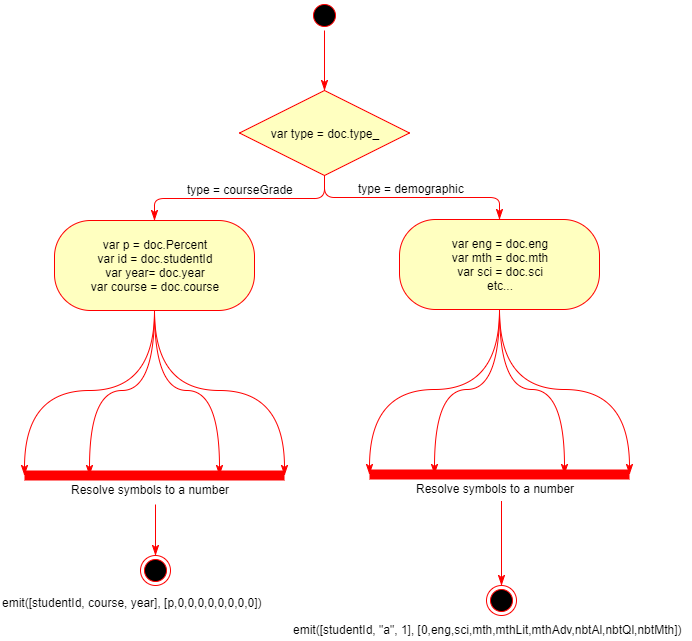
\includegraphics[scale=0.35]{./resources/figures/activity-diagram-1.png}
    \end{mdframed}
    \caption[Result 1 Map function]{\textbf{Figure \ref{result-1-map-fn}: Activity diagram showing logic Map function logic for Results 1 \& 2.} This logic is applied to every document during index calculation (excluding documents with an \_id of ``\_design/*'').}
    \label{result-1-map-fn}
\end{figure}

\subsection*{The List function}
The list function is used to iterate over the results of the MapReduce view, and transform the JSON structure of the view return into a CSV. The list function is included in the appendix (see \ref{result-1-list}). The logic is fairly straight forward; The list function is called via HTTP, specifying the view in the URL, along with the options to group map output by key (at exact level) and to use the reduced result set. The List function first emits a row of headers, as defined in the function itself, and then iterates over the keys in the MapReduce index. For each key, the List function emits a string of comma separated values followed by a newline char according to the RFC 4180 specification. This allows for CSV's to be created and downloaded incrementally allowing for iteration over huge MapReduce indexes.

As mentioned previously List functions are likely to become deprecated in CouchDB. As such it would be better practice to replicate the logic of the List function in a node.js (or alternative) application. If this were to be done, the logic involved in producing a CSV from the MapReduce results would remain the same.
